\subsection{\texorpdfstring{$y''+cy = 0$}{y''+cy = 0}}
Indem $a$ verschwindend klein gew"ahlt wird, entsteht
\begin{equation}
	y''+ cy = 0.
	\label{eq:wellen:lineareDGL}
\end{equation}

Diese lineare Differentialgleichung kann mit Hilfe des charakteristischen 
Polynoms
\begin{equation*}
	p(\lambda) = [(\lambda+\mu)^2+\omega^2] = 0
\end{equation*}
dessen L"osungen
\begin{equation*}
	\begin{split}
		y_1 &= C_1e^{-\mu x}\cos(\omega x) \\
		y_2 &= C_2e^{-\mu x}\sin(\omega x)
	\end{split}
\end{equation*}
sind, gel"ost werden.

Angewandt auf die Gleichung \ref{eq:wellen:lineareDGL} ergibt sich nun zu
\begin{equation*}
	\begin{split}
		p(\lambda) &= [(\lambda+0)^2+\sqrt{c}^2] = 0 \\
		\Leftrightarrow p(\lambda) &= [\lambda^2+c] = 0,
	\end{split}
\end{equation*}
was uns nun
\begin{equation}
	y(x) = C_1 \cos(\sqrt{c}x) + C_2 \sin(\sqrt{c}x)
	\label{eq:wellen:loesunglinearedgl}
\end{equation}
als L"osung ergibt.

Um die Konstanten $C_1$ und $C_2$ zu bestimmen m"ussen die Anfangsbedingungen 
$a_0$ und $a_1$ bekannt sein. Damit die Abh"angigkeit auf gezeigt werden kann, 
wird zuerst die erste Ableitung der L"osung (\ref{eq:wellen:loesunglinearedgl}) 
aufgestellt werden.

\begin{equation}
	y'(x)=-C_1 \sqrt{c} \sin(\sqrt{c}x) + C_2 \sqrt{c} \cos(\sqrt{c}x)
\end{equation}

Die Werte von $y(0)$ und $y'(0)$ sind jeweils durch $a_0$ beziehungsweise $a_1$ 
gegeben. Setzt man nun $x = 0$ ein, ergibt sich f"ur $C_1$ und $C_2$
\begin{equation}
	\begin{split}
		y(0) = C_1 = a_0 &\Leftrightarrow C_1 = a_0 \\
		y'(0) = C_2 \sqrt{c} = a_1 &\Leftrightarrow C_2 = \frac{a_1}{\sqrt{c}}.
	\end{split}
\end{equation}

Eingesetzt in die L"osungsgleichung(\ref{eq:wellen:loesunglinearedgl}) erhalten 
wir nun
\begin{equation*}
	y(x) = a_0 \cos(\sqrt{c}x) + \frac{a_1}{\sqrt{c}} \sin(\sqrt{c}x), \qquad c 
	> 0
\end{equation*}
und
\begin{equation}
	\begin{split}
		y(x) &= a_0 \cos(i\sqrt{|c|}x) + 
		\frac{a_1}{i\sqrt{|c|}}\sin(i\sqrt{|c|}x), \qquad c < 0\\
		\Leftrightarrow
		y(x) &= a_0 \cos(i\sqrt{|c|}x) - 
		i\frac{a_1}{\sqrt{|c|}}\sin(i\sqrt{|c|}x)\\
		\Leftrightarrow
		y(x) &= a_0 \cosh(\sqrt{|c|}x) + 
		\frac{a_1}{\sqrt{|c|}}\sinh(\sqrt{|c|}x).
	\end{split}	
\end{equation}
Der letzte Umformungsschritt ergibt sich aus der Definition von $\cosh$ und 
$\sinh$:
\begin{equation*}
	\begin{split}
		\sinh(x) &= \frac{1}{2} (e^x - e^{-x}) = -i \sin(ix)\\
		\cosh(x) &= \frac{1}{2} (e^x + e^{-x}) = \cos (ix)
	\end{split}
\end{equation*}

Die gefundenen L"osungen k"onnen auch graphisch best"atigt werden. Sei es f"ur 
positve $c$ in der Abbildung \ref{fig:wellen:sinh-cosh} oder f"ur negative $c$ 
in Abbildung \ref{fig:wellen:sin-cos}.

\begin{figure}
	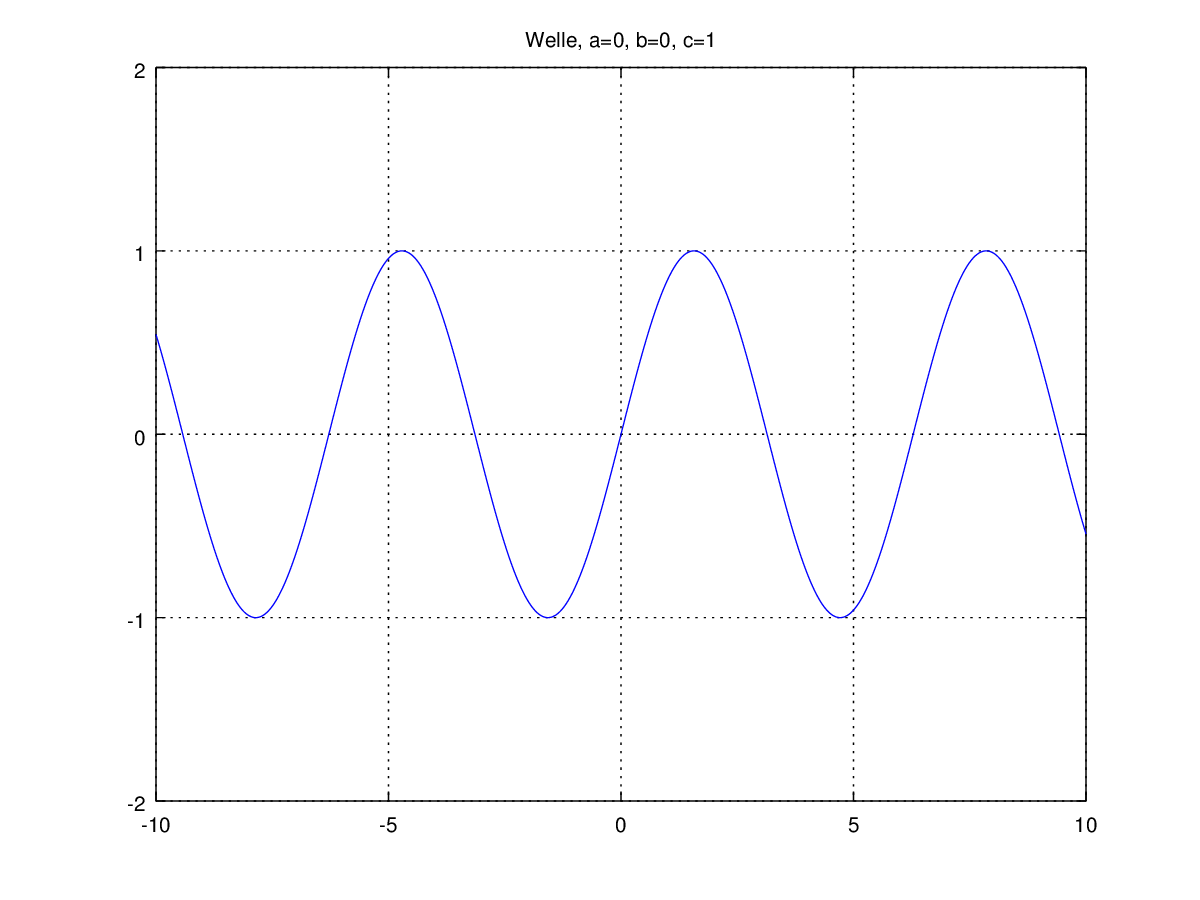
\includegraphics[width=0.5\hsize]{./wellen/images/basicfunctions/sin.png}
	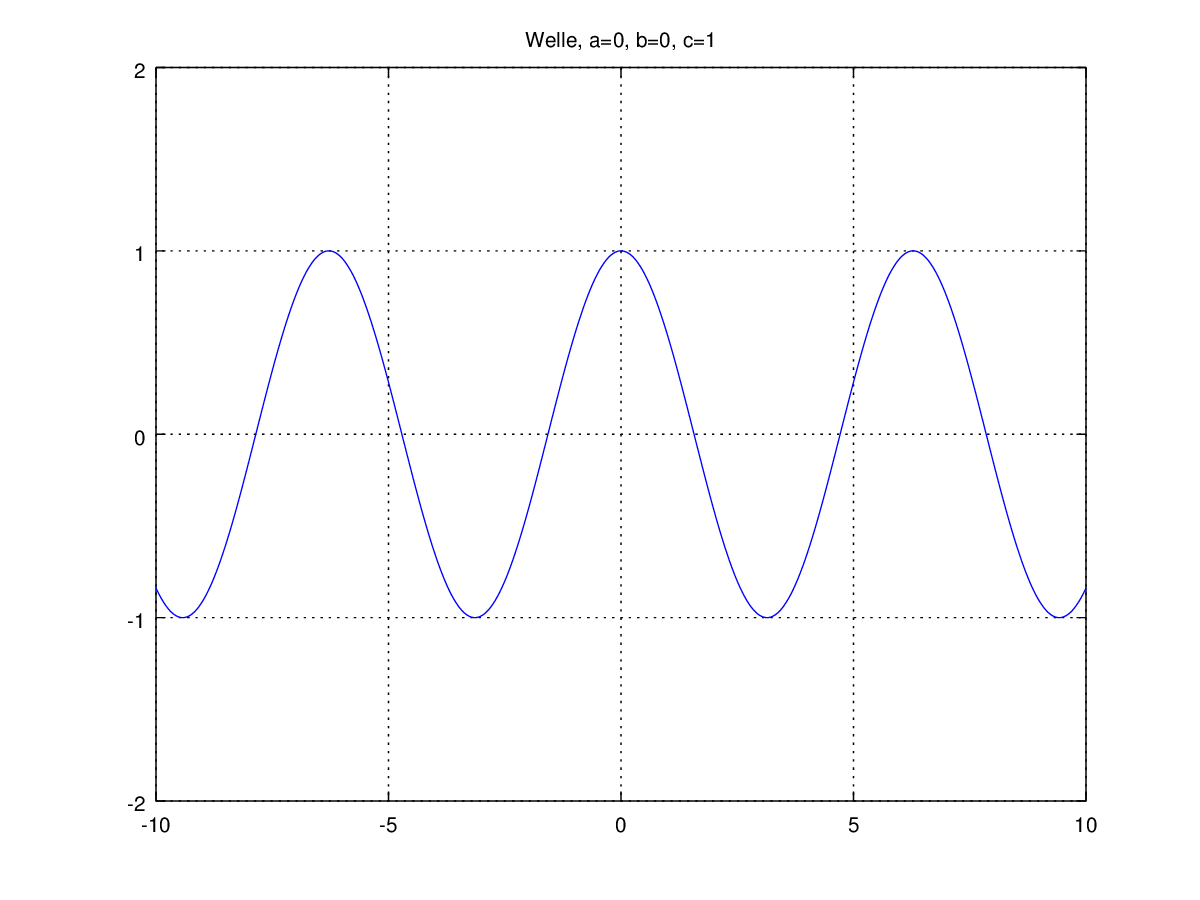
\includegraphics[width=0.5\hsize]{./wellen/images/basicfunctions/cos.png}
	\caption{$\sin$ (l.) und $\cos$ (r.)}
	\label{fig:wellen:sin-cos}
\end{figure}

\begin{figure}
	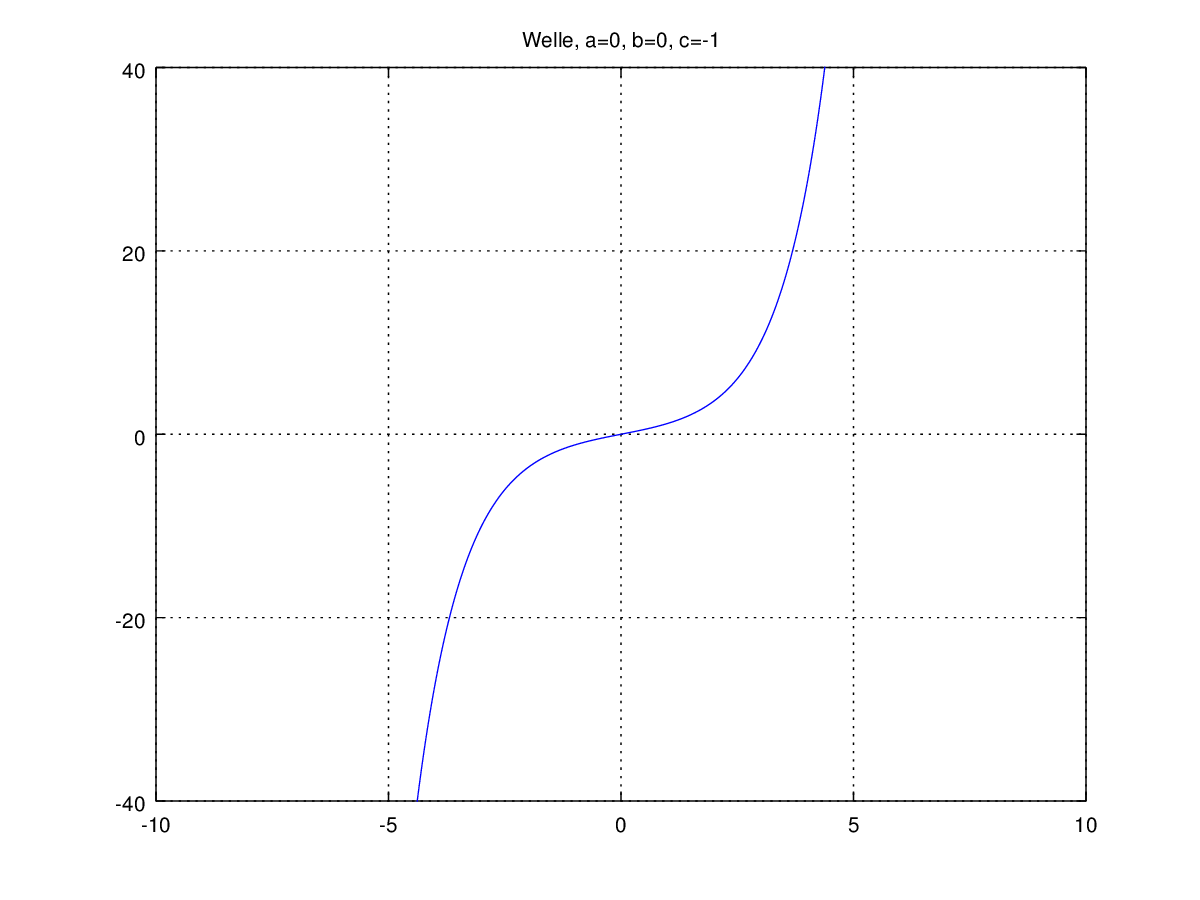
\includegraphics[scale=0.35]{./wellen/images/basicfunctions/sinh.png}
	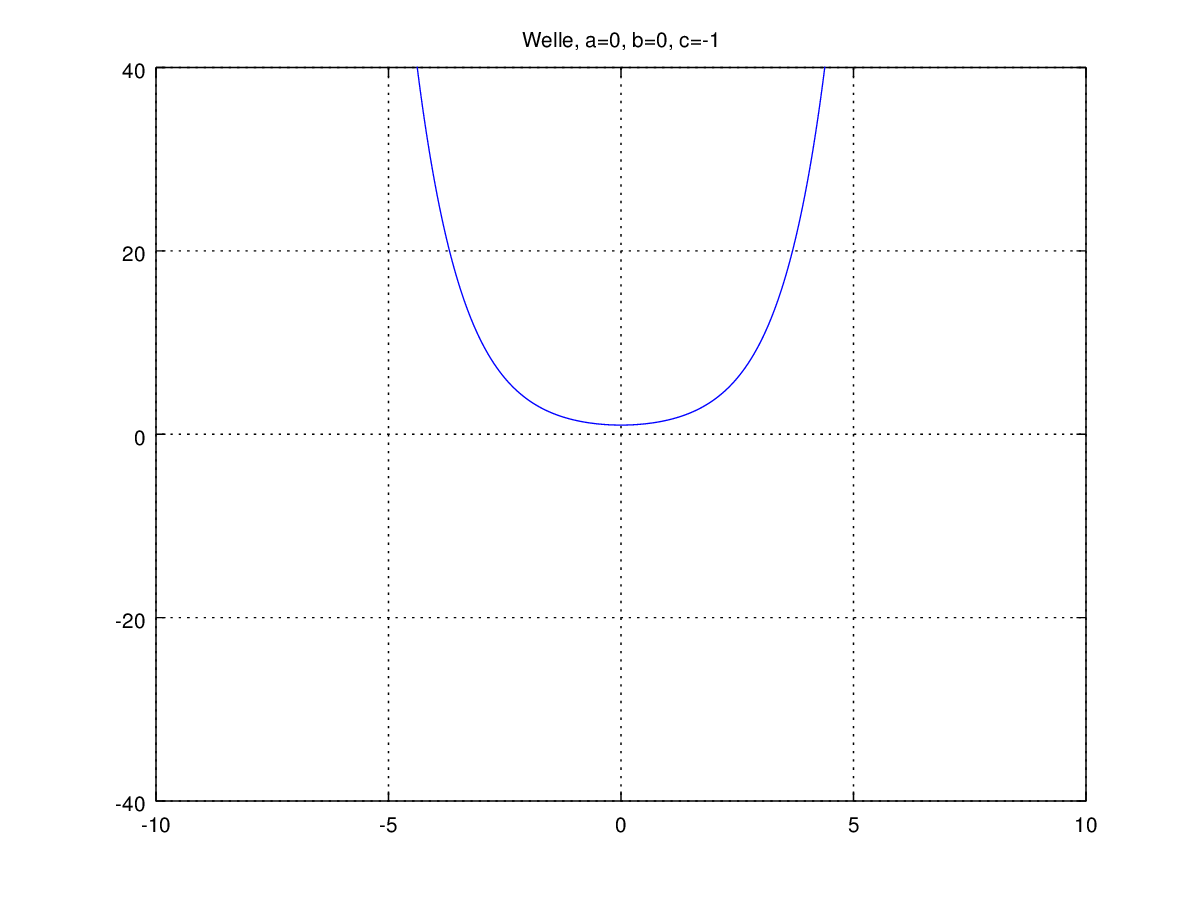
\includegraphics[scale=0.35]{./wellen/images/basicfunctions/cosh.png}
	\caption{$\sinh$ (l.) und $\cosh$ (r.)}
	\label{fig:wellen:sinh-cosh}
\end{figure}